\documentclass[english]{ntnuthesis}

% Make index:
\usepackage{makeidx}

\usepackage{hyperref}
\usepackage[T1]{fontenc}
%\usepackage[latin1]{inputenc}
\usepackage[english]{babel}
\usepackage{appendix}
\usepackage{textcomp}
\usepackage[binary,squaren]{SIunits}
\usepackage{amsmath, amsfonts, amssymb}
\usepackage{graphicx, subfigure, wrapfig}
\usepackage{listings}
\usepackage{multirow}
\usepackage[subfigure]{tocloft}
\usepackage{acronym}
\usepackage{lmodern}
\usepackage{pdfpages}

% MATLAB: load package with ``framed'' and ``numbered'' option.
\usepackage[framed,numbered]{mcode}

\usepackage{algorithm,algorithmicx,algpseudocode}
\algnewcommand\algorithmicto{\textbf{to}}

% Do not use bullets in un-numbered lists:
\renewcommand{\labelitemi}{\normalfont\textendash}
\renewcommand{\labelitemii}{\normalfont\textperiodcentered}

% Do not use dot after speaches in numbered lists:
\usepackage[pointlessenum]{paralist}

% Accept comma as fraction separator in math expressions
% (This package is much smarter than the icomma-package.)
\usepackage{ncccomma}

% Macro for microseconds
\newcommand{\us}{\,$\mu$s}

% Define AVR32 assembly
\lstdefinelanguage{avr32asm}{
morekeywords={lddpc,mov,st.w,cp.w,cp.b,bfextu,breq,
brne,rete,sub,rjmp,lsl,lsr,com,st.w,ld.w,csrf,mtsr,
rcall,reteq,br,ret,.int,.include,.globl},
  sensitive=false,
morecomment=[l]{//},
morecomment=[s]{/*}{*/},
alsodigit={.},
}

\lstloadlanguages{c, c++, avr32asm, vhdl}

% Used with the make index package
\makeindex

\begin{document}
\hyphenpenalty=8000
\exhyphenpenalty=8000
% Write how to divide long words:
\hyphenation{temp-tation}

\frontmatter

\title{Dual RISC-V cores for glitch protection}

\author{ Jarl Magnus Sæbø }
\degreetype{MSc in Electrical systems design}

\maketitle
%\includepdf{titlepage}
%\includepdf{problemdes}
% Insert page number
\setcounter{page}{5}
\chapter{Abstract}

This project aims at using the CV32E40S RISC-V CPU in a dual-core lockstep mechanism as a way of doing glitch protection. The purpose of this research is to determine whether this simple measure can replace pre-existing and much more complex security features. By proving the effectiveness of this new hardware architecture, it paves the way for developers to simplify their designs and speed up the development of future CPUs. In addition, this project aims at broadening the public knowledge about secure CPU design, as this topic is largely kept a secret by the major players in the industry. 

To address this, all research was done on an open-source RISC-V core. This core contains a lot of complex security features, which were found to add a somewhat significant amount of resource usage. By simply disabling one of the many security features the overall performance of the system could be increased by 5\%. To compare the quality of the dual-core setup with the existing setup, they were both subjected to different types of simulated glitch attacks while running a simple test program. From these tests we found that the dual-core setup was just as capable of detecting errors, and even surpassed the existing setup in some cases. This means that it is a simple and viable alternative for researchers aiming to secure their hardware against glitch attacks. 

To advance this research, the next phase involves fabricating an actual chip based on the proposed architecture and assessing its resilience against various real-world glitch attacks. Specific focus will be given to electromagnetic fault injection, voltage manipulation, and clock glitching techniques, which pose substantial threats to modern computing systems. This comprehensive evaluation will provide important insights into the practical viability of the dual-core lock-step mechanism as a security solution for RISC-V cores.

\chapter{Preface}
I would like to thank....


\cleardoublepage

% Remove parskip for toc
\setlength{\parskip}{0ex plus 0.5ex minus 0.2ex}
\thispagestyle{fancyplain}
\setcounter{tocdepth}{2}
\tableofcontents


\cleardoublepage
\listoftables
\cleardoublepage
\listoffigures
\cleardoublepage
\renewcommand{\lstlistlistingname}{Source code}
\lstlistoflistings

\chapter{List of abbreviations}
\begin{acronym}
\acro{ADC}{Analogue to Digital Converter}
%\acro{}{}
\end{acronym}

\cleardoublepage

\mainmatter

\chapter{Introduction}
\label{intro} 

Modern integrated systems and other programmable electronics often have safety-measures built in to avoid unintended behaviour, whether it be accidental or from an external source. These safety measures typically only address software or firmware issues, leaving systems unprotected against hardware-induced faults, known as glitch attacks. These attacks are able to bypass robust software and firmware security measures given the right method of attack. Interestingly, despite the importance of glitch protection, it only started gaining attention after practical glitch attacks first made their appearance in 2002 through an optical fault attack\cite{trouchkine2019fault}. 

In the world of computer architecture, many aspects remain closely guarded secrets, including preventive measures against glitch attacks. This secrecy often makes these preventative measures inaccessible to the public. Over recent years there has been a large shift away from this secrecy as more and more researchers and companies use the \textit{RISC-V} instruction set architecture (ISA)\cite{riscv_manual}. This architecture is open source, allowing anyone with the right knowledge and motivation to create their own central processing unit (CPU). One group of people doing this is the \textit{OpenHW Group} who have developed several publicly available RISC-V CPUs over recent years. One of these is the \textit{CV32E40S}, which is a core mainly focused on safeguarding against glitch- and side-channel attacks\cite{cv32e40s_manual}.

While the \textit{CV32E40S} has a proven to be able to detect glitch attacks, it comes at a cost in performance. Often the methods used to protect against attacks are complex and increase the execution time and power needed for the CPU to perform its given tasks. This project investigates the possibility of replacing some of the security features of the \textit{CV32E40S} in favour of running two CPUs in a \textit{Dual-Core Lockstep} (DCL) mechanism instead to increase throughput and simplicity. Henceforth the core using the DCL mechanism is reffered to as the \textit{CV32E40DC}. 

\section{Sustainability}
\label{sec:sustainability}

Out of the 17 sustainability goals of the United Nations\cite{un}, at least two can be considered highly relevant for this project. 

\begin{itemize}
    \item \textbf{Goal 9:} Build resilient infrastructure, promote sustainable industrialization and foster innovation.
    \item \textbf{Goal 17:} Revitalize the global partnership for sustainable development.
\end{itemize}

The goal of this project is to investigate a new way of possibly making components more resilient against attacks and exploits. This fits into \textit{goal 9}. In addition, this project works to increase the knowledge around an open source project. Being open source means anyone in the world can access all parts of the code. This is relevant for promoting \textit{goal 17} of revitalizing global partnership for sustainable development. 

\section{The use of AI}
\label{sec:AI}

The AI chat bot ChatGPT made by \textit{Open AI}\cite{chat} was used as an academic tool when working on this project. Its main use was to offer possible ways to restructure parts of the text that could be difficult to understand or where the point did not come across clearly. For example, I had the following text where the word "them" could be ambiguous: 

\begin{lstlisting}
Restructure this sentence so its more clear what "them" is: 
In the world of computer architecture, many aspects remain closely guarded
secrets. This secrecy extends to preventive measures against such 
attacks, making them often inaccessible to the public.
\end{lstlisting}



In addition it was used to generate code that would otherwise be tedious to write. This includes for example SystemVerilog code where two modules with large interfaces are connected. 
\chapter{Problem Definition}
\label{chap2}

Modern integrated systems and other programmable electronics very often have several safety-measures built in to avoid unintended behaviour, whether it be accidental or from an external source. These safety measures are often only handled on the software or firmware level, but for a long time hardware induced faults, glitches, have been a concern that has gained less focus even though they are capable of bypassing software security measures given the right attacker. Interestingly, despite the relevance of glitch protection, it only started gaining attention after practical glitch attacks first made their appearance in 2002 through an optical fault attack\cite{trouchkine2019fault}. In the world of computer architecture, many aspects remain closely guarded secrets. This secrecy extends to preventive measures against such attacks, making them often inaccessible to the public. This paper aims to supply the public with a good understanding of a new way to do glitch protection, on the open source RISC-V instruction set architecture (ISA). 

The RISC-V architecture has gained a lot of traction in both academia and industry due to its modular design and adaptability\cite{source2}. However, due to the nature of open source resources, RISC-V systems are often more susceptible to glitch attacks as hackers can research the ISA in depth to find errors\cite{isa_exploit}\cite{trouchkine2019fault}. In addition to this, the actual chips made with the RISC-V architecture will still be susceptible to more common attacks like electromagnetic fault injection (EMFI) or voltage- and clock-glitching. 

The openHW group has developed an instruction set extension (ISE) 'Xsecure' which contains several extra features aimed at stopping side-channel attacks as well as glitches. To prevent glitches the extensions introduces Error Correcting Code (ECC) for the registers and hardening of both the Program Counter (PC) and the Control and Status Registers (CSRs). These additions can slow down the performance of the CPU , increase the power usage and increase the over all complexity of the core. This paper researches the possibility of using dual RISC-V cores and comparing the entire state of both cores to provide redundancy and thereby glitch protection, without significantly impacting the power, performance and area (PPA) in a negative way. 

The current way of doing glitch protection that is used by 'Xsecure' also allows the user to sometimes get a specific error message saying where and what things went wrong. This feature is however not able to do this for all major alerts or errors. The proposed dual core setup might be able to give detailed errors every time as it is possible to know exactly which area of the cores that are not coinciding. 

Introducing a dual-core setup offers potential glitch protection via redundancy. However, the feasibility, overheads, synchronization mechanisms, and actual effectiveness of such a strategy needs thorough examination. In addition, the strategies for detection of a glitch, switch-over mechanisms, and potential recovery strategies need to be explored. An exploration of where and how glitches typically affect RISC-V cores is crucial. From other literature it is apparent that most glitches are induced outside of the CPU pipeline itself, and instead on larger area intensive components like data busses or register files/caches\cite{emfi_injection}. Because it is not feasible to validate the state of caches and register files at all times it is necessary to explore whether a dual core setup will be able to stop or register these types of glitches also.  
%4. Scope of the Problem:

%System Vulnerabilities: An in-depth understanding of where and how glitches typically affect RISC-V cores is crucial. This entails both functional and performance impacts.
%Dual Core Strategy: Introducing a dual-core setup offers potential glitch protection via redundancy. However, the feasibility, overheads, synchronization mechanisms, and actual effectiveness of such a strategy need thorough examination.
%Protection Mechanisms: Beyond the mere introduction of dual cores, the strategies for detection of a glitch, switch-over mechanisms, and potential recovery strategies need to be explored.
%5. Objectives:

%The primary objectives for this project include:

%Conducting a vulnerability analysis of single-core RISC-V systems concerning glitches.
%Designing a dual-core RISC-V system prototype aiming for glitch protection.
%Evaluating the effectiveness of the dual-core setup in real-world scenarios and benchmark tests.
%Proposing additional countermeasures or strategies, if needed, to enhance glitch protection further.
%6. Significance:
%By addressing the problem defined, this project aims not only to enhance the reliability of RISC-V based systems but also to contribute to the broader realm of glitch protection in electronics. With the ever-increasing adoption of RISC-V in various applications, ensuring its robustness against glitches will be paramount for many industries.


%Start with a Clear Heading: Begin your report with a heading that clearly states "Background" or "Introduction" to let readers know where to find this information.

%Provide an Overview: Begin by providing a brief overview of the project, including its title and purpose. You can mention what the project aims to achieve or the problem it intends to address.

%Contextualize the Project:

%Explain the broader context in which the project exists. Discuss any relevant industry trends, challenges, or issues that the project is responding to.
%Mention any external factors or events that have prompted the need for the project.
%If the project is part of a larger initiative or program, briefly introduce that program and explain how your project fits into it.
%Historical Background:

%Provide historical information if relevant. Explain how this project came into consideration, including any past efforts or developments leading up to it.
%If there are key milestones or events that are crucial to understanding the project's origins, mention them.
%State the Problem or Opportunity:

%Clearly state the problem or opportunity your project aims to address. Use data or facts to support your claims.
%If applicable, describe the significance of the problem or opportunity, such as its impact on the organization, stakeholders, or the community.
%Objective and Scope:

%Outline the specific objectives and scope of the project. What are you trying to achieve, and what are the boundaries or limitations of the project?
%Explain why these objectives are important and how they relate to solving the identified problem.
%Review of Relevant Literature:

%If there's existing research or literature relevant to your project, briefly mention it. This shows that you've conducted a literature review and are building upon prior knowledge.
%Highlight any gaps or areas where your project adds value or addresses shortcomings in existing research or practices.
%Cite Sources: Make sure to provide proper citations for any data, statistics, or information you use in this section.

%Keep it Concise and Engaging: While providing all necessary information, avoid making the background section overly long. Keep it engaging and focused on the most crucial information.

%Transition to the Next Sections: Conclude the background section by smoothly transitioning into the next sections of your report, such as the objectives, methodology, or project plan.

%Remember to tailor the background section to your specific project and audience. Your goal is to provide a comprehensive but concise overview that sets the stage for the reader to understand the significance and context of your project.

\chapter{Background}
\label{chap3}

\section{What are glitch attacks?}

Glitch attacks can be divided into two main categories: invasive (e.g., decapsulating the chip\cite{intro_to_hw_hacking}) and non-invasive attacks (e.g., electromagnetic fault injection (EMFI), voltage- and clock-glitching). Often times software and firmware security measures can only protect against non-invasive glitches, as protecting from invasive glitches often require hardware modifications\cite{glitchresistor}. Due to the nature of invasive attacks, it is beyond the scope of this project to defend against them. These often aim at tampering with Read-Only Memory (ROM) or Boot-loaders on Printed Circuit Boards (PCBs), and are not effective against more complex systems like a Central Processing Unit (CPU) or a System on Chip (SoC). 

Non-invasive glitches can be performed as long as an attacker has access to a device. However, there is quite a lot of procedural vulnerability discovery that has to be done before an attack can be performed. In the case of EMFI the chip has to be repeatedly exposed to electromagnetic interference during execution, to then determine which areas are most vulnerable to attacks\cite{emfi_injection}. An example of this being performed on the BCM2837 SoC can be seen in \autoref{fig:emfi_map}\cite{emfi_injection}. 

Voltage- or clock-glitching can be performed as long as there is some way to access these signals externally. Voltage-glitching often requires the removal of power filtering capacitors to gain more fine-grained control over a processor's voltage input. However, both of these methods require very precise timing by an attacker. This is why specialized tools such as the \textit{ChipWhisperer}\cite{chipWhisperer} are needed, as they allow extremely accurate fault-injection. These days it is also possible to perform effective glitch attacks with simple components in conjunction with a cheap Field Programmable Gate Array (FPGA) which outputs precise triggers\cite{hole_in_soc}. 

\begin{figure}[h!]
    \centering
    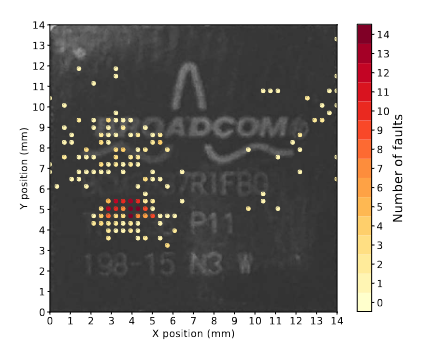
\includegraphics[scale=0.5]{docs/images/emfi_error_map.png}
    \caption{EMFI BCM2837 sensitivity map (dot size is not corralated with probe size.)\cite{emfi_injection}.}
    \label{fig:emfi_map}
\end{figure}

Voltage-glitching is performed by momentarily dropping the supply voltage during execution of critical operations. Clock-glitching is performed by altering clock timing to violate setup and hold time requirements of the hardware\cite{intro_to_FI}. The results of glitching cannot always be predicted, however they mainly result in skipped or repeated CPU instructions, incorrect evaluation of CPU instructions or corrupt reads from memory devices\cite{intro_to_FI}. In general these faults can occur at any stage in the execution pipeline. 

% Glitch attacks have over recent years become a more common and greater threat. Due to the nature of how these attacks are carried out, they are often a very affordable way to exploit hardware. Attackers have easy access to open source resources like the the 'ChipWhisperer Lite' which allows for easy access to hardware glitching tools as well as side channel analysis\cite{chipWhisperer}. In addition to this, FPGAs can be used to inject precisely timed faults as long as an attacker has access to the supply voltage or clock on a chip\cite{hole_in_soc}. 

\section{The need for glitch protection}

For many years the world of CPU design has been hidden from the public due to the strict secrecy producers have around their products. While this limits what the general public can know, it also means that a potential hacker would have a much harder time if they wished to exploit how the ISA of a chip is designed. Due to the nature of open source projects, this is a larger vulnerability for products based on a RISC-V architecture. An example of direct exploitation of the architecture was shown during the 'DEFCON' conference in 2019\cite{isa_exploit}. Here it was demonstrated that triggering an exception during boot of a RISC-V chip would lead to an 'exception loop'. This was because the Machine Trap Vector (MTVEC) had no base address before boot (e.g., it was set to 0x0). Pointing to this address is permitted in the ISA, and doing so will trigger an exception. This means that triggering an exception before boot leads to the exception handler pointing to an illegal address, which again triggers an exception and this continues forever. Handling of exceptions happens first at the highest privilege mode (Machine mode), which means that the chip is also stuck in this mode. 

The RISC-V architecture is designed with some key security features in mind. One of these are the previously mentioned privilege levels. These are in descending order: machine (M-mode), hypervisor (H-mode), supervisor (S-mode) and user mode (U-mode). A higher privilege mode can access all the functions used in a lower privilege mode\cite{source2}. Other key security features in the RISC-V architecture are the physical memory protection (PMP), which controls memory accesses, and the use of a trusted execution environment (TEE). The TEE is meant to ensure that code and data loaded into this environment are protected with respect to confidentiality and integrity. However, as shown in (Nashimoto et al. 2020) the integrity of TEEs can also be bypassed using clock-glitching\cite{source2}.

%\section{Previous Approaches to glitch protection}
\section{CV32E40S by the OpenHW group}
\label{sec:cv32}

The previously mentioned security measures do a decent job at protecting hardware against malicious attacks. However, the need for more security features has been required and therefore the \textit{OpenHW} group developed the \textit{CV32E40S}. This is a 4-stage in-order 32-bit RISC-V processor core with the main intention of ensuring secure operation\cite{cv32e40s_manual}. This core has the same privilege modes and PMP as described to ensure a TEE. There are however implemented extra security features and an Instruction Set Extension (ISE), \textit{Xsecure}. The CV32E40S started out as a fork of the CV32E40P which is another RISC-V processor made by the OpenHW group. The  


\subsection{Xsecure Extension}
\subsubsection{Hardened PC}
\subsubsection{Hardened CSR}
\section{Limitations of glitch protection}
\label{sec:limits}

\begin{itemize}
    \item High logic cost 
    \item Slower execution of certain pipeline stages
    \item Lower throughput 
    \item A typical way of doing fault injection is though EMFI attacks which target larger components like caches or other memory components.
    How can we prevent these? Comparing the state of the entire chache is not viable, and thus we must allow a fault to persist in 
    memory untill it is read or used in one of the cores.
\end{itemize}
\section{The dual core proposition}
\section{Rationale for this study}


\chapter{Experimental}
\label{chap4}

\section{Methodology and theory}
\label{sec:method}

\subsection{How are the different layouts tested?}
\subsubsection{Synthesis tool - Which one is used?}
\subsubsection{How is fault injection done in sumlation?}
\subsection{How are results from fault injection compared between the different setups?}

\section{Limitations}
\label{sec:limit}

\section{Choices / Findings}
\label{sec:choice}
\chapter{Results and Analysis}
\label{chap5}

To perform the tests described in \autoref{tab:instr_skip_test} we follow the steps described in \autoref{subsec:sim_glitch}.

\section{PPA comparison}
\label{sec:synth_comparison}

Results of synthesis of both cores as well as number of cycles needed to complete the test program in \autoref{app:helloworldC} is shown in \autoref{tab:ppa_results}. The relative difference from the single core to dual-cores is shown in the table.

\begin{table}[h]
\centering
\caption{PPA results from simulation and synthesis of both setups.}
\label{tab:ppa_results}
\begin{tabular}{c|ccc}
\toprule 
Setup & Area[$pm^2$] & Power[$\mu W$] & Clock Cycles\\
\midrule
\rowcolor{black!20} CV32E40S & 63121.093 & 113.007 & 18424\\
CV32E40S Dual-Core & 65214.732[$+3.3\%$] & 144.482[$+27.9\%$] & 17446[$-5.3\%$] \\
\bottomrule
\end{tabular}
\end{table}

\section{Instruction Skipping}
\label{sec:instr_skip_result}

\subsection{CV32E40S}
\label{subsec:single_instr_skip}

\subsubsection{Skipping function call}

 From the log file, we can see that the \textit{c.jal} instruction is logged at 1752ns. To skip this instruction the program counter needs to be skipped in the \textit{IF} stage, which is 3 cycles before \textit{WB}. The system clock has a period of 3ns, meaning the glitch is injected at 1743ns. The \textit{c.jal} is located at the address: \textit{0x0000044c}. Forcing the program counter to the next address \textit{0x0000044e} for a duration of 3ns will simulate an instruction skip. The address of the next instruction is only 2 away because the \textit{jal} is a 16-bit compressed instruction.

Glitching of the core was done successfully. The waveforms from simulation are shown in \autoref{fig:instr_skip_single_wave}. From the figure one can see that the glitch is detected immediately. 

\begin{figure}[h!]
    \centering
    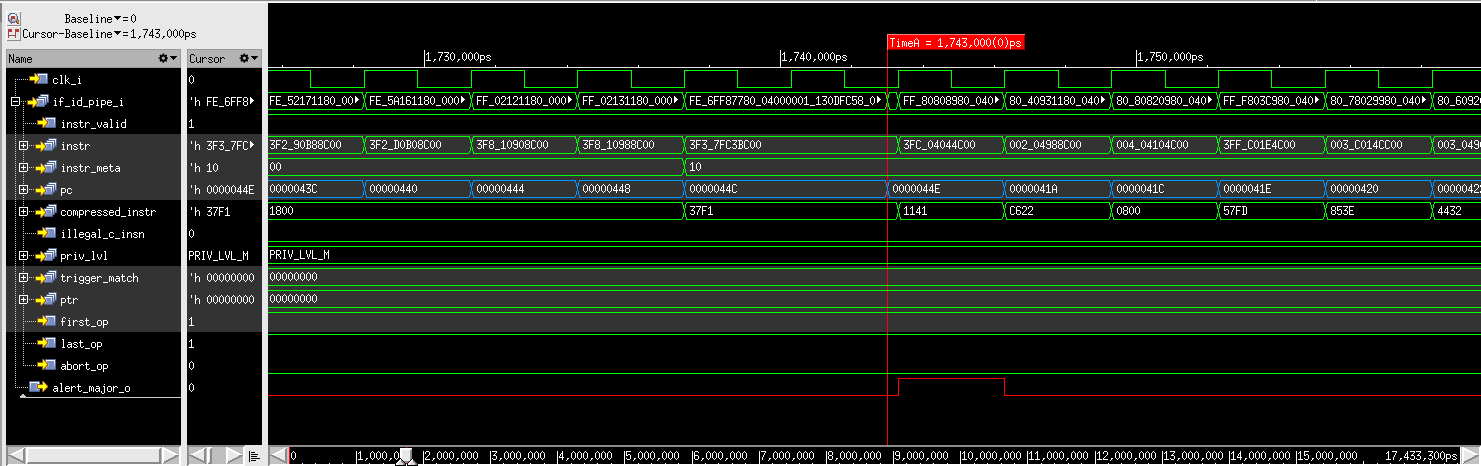
\includegraphics[width=\textwidth]{docs/images/instr_skip_glitch_injection_single_core.png}
    \caption{Waveforms from simulated instruction skip on CV32E40S.}
    \label{fig:instr_skip_single_wave}
\end{figure}

\subsubsection{Skipping out of while loop}

From the log file, we can see that the \textit{c.j} instruction is called 10 times. We skip the one logged at 1833ns. To skip this instruction the program counter needs to be skipped in the \textit{IF} stage, which is 3 cycles before the \textit{WB}. The \textit{c.j} is located at \textit{0x0000047a}. Forcing the program counter to the next address \textit{0x0000047c} for a duration of 3ns will simulate an instruction skip. This address is only 2 away because the \textit{j} is a 16-bit compressed instruction. 

Glitching out of the while loop was not successful. This is possibly due to other branch instructions from the loop that are also inside the pipeline. The attempted instruction skip is still detected and a major alert is raised. This can be seen in the simulation waveforms in \autoref{fig:instr_skip_loop_single_wave}. 

\begin{figure}[h!]
    \centering
    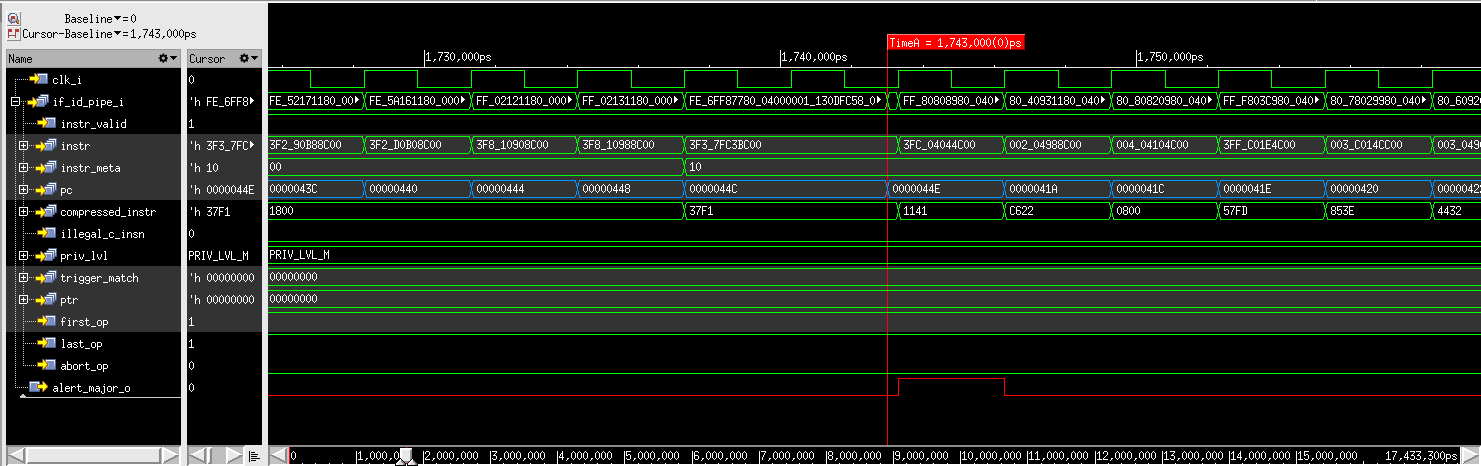
\includegraphics[width=\textwidth]{docs/images/instr_skip_glitch_injection_single_core.png}
    \caption{Waveforms from simulated instruction skip on CV32E40S.}
    \label{fig:instr_skip_loop_single_wave}
\end{figure}

\subsubsection{Skipping directly to end}

As mentioned earlier, an attacker can potentially glitch directly to the end of the program if they have some way of manipulating the code in the boot-loader. To simulate this, the program counter is forced to the address of the instruction after the while loop, \textit{0x00000482}. This force happens as soon as the main program is entered, which is at 1737ns.

This glitch attack was not successful. However, no major alert was raised by the core as can be seen in \autoref{fig:direct_skip_single_wave}. This glitch therefore bypassed the PCH feature. 

\begin{figure}[h!]
    \centering
    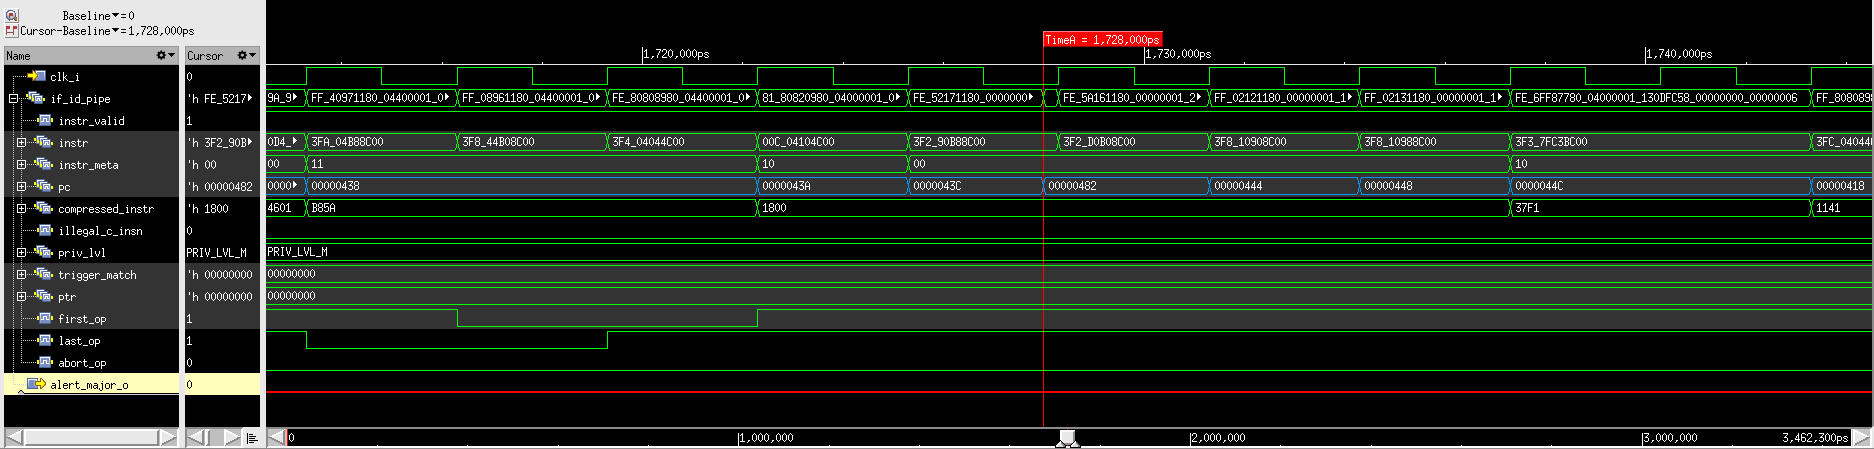
\includegraphics[width=\textwidth]{docs/images/direct_skip_single_core.png}
    \caption{Waveforms from simulated direct instruction skip on CV32E40S.}
    \label{fig:direct_skip_single_wave}
\end{figure}

\subsection{Dual-Core Lockstep}
\label{subsec:dual_instr_skip}

\subsubsection{Skipping function call}

The call to the \textit{c.jal} instruction occurs at 1707ns. The program counter is glitched to the address \textit{0x0000044e}. The 

\begin{figure}[h!]
    \centering
    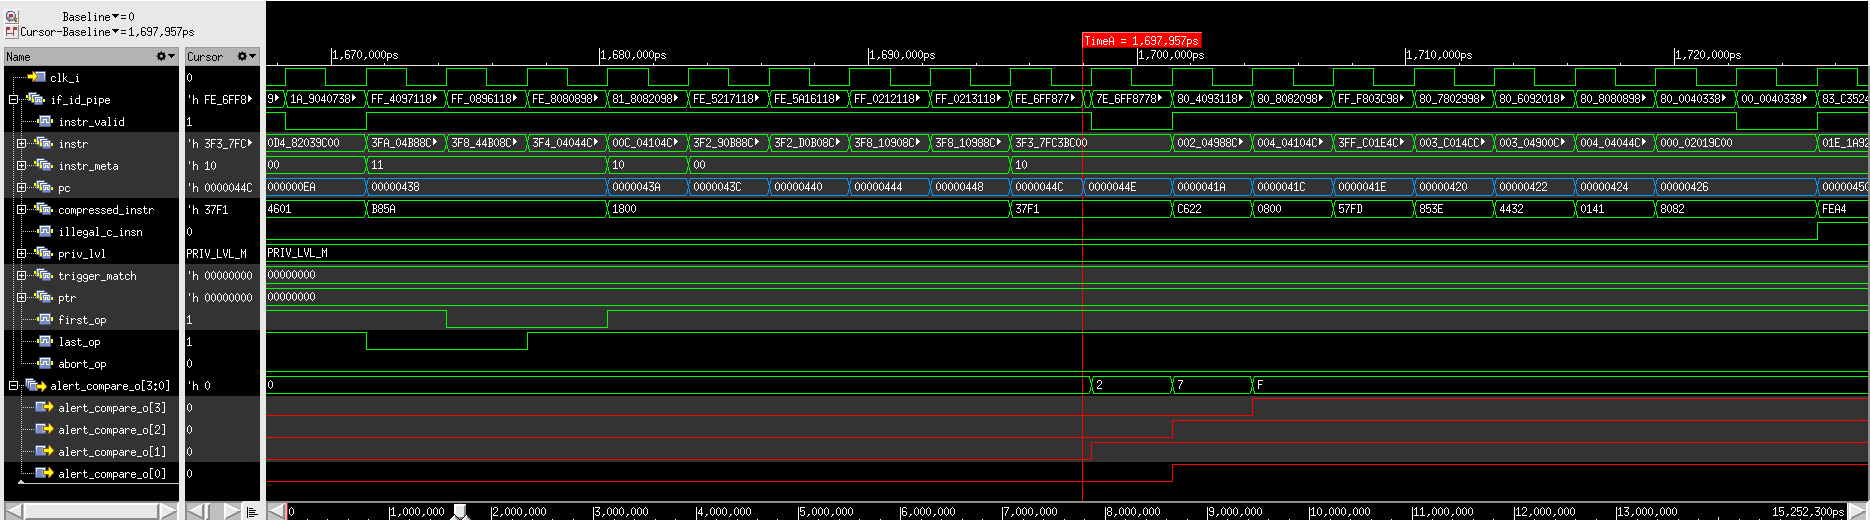
\includegraphics[width=\textwidth]{docs/images/instr_skip_dual_core.png}
    \caption{Waveforms from simulated instruction skip on Dual-Core Lockstep setup.}
    \label{fig:direct_skip_single_wave}
\end{figure}


\subsubsection{Skipping out of while loop}

The call to the \textit{c.j} instruction occurs first at 1782ns. The program counter is glitched to the address \textit{0x0000047c}.

\subsubsection{Skipping directly to end}

The call to the \textit{main} function occurs at 1689ns. The program counter is glitche dto the address \textit{0x00000482}.


\section{Coverage Test}
\label{sec:cov_test_result}



\textbf{Instruction to be glitched:}
\begin{lstlisting}
       30003.000 ns | 0000672c | memchr syscalls.c 379 - beq x14,x10,66b4 <memchr+0x3c>
\end{lstlisting}

In order to glitch the loop we need to make the program skip the instruction that happens at 29991.000 ns. This is a bne instruction that keeps us in the loop. Next instruction occurs at 29997 and we must therefore chang ethe program counter before this. 

Glitch 6734 to 673c

Count lagret i x8 
Verdien 10 lagret i x9

\section{Layout comparisons}

\subsection{Can this be implemented in read hardware?}
\begin{itemize}
    \item Compare performance 
    \item Compare area
    \item Compare Timing 
    \item Compare simulated power usage
    \item Compare glitch detection
\end{itemize}

\section{Why is this solution good/bad}

Synthesis results no pc hardening and dual core:

Area: 65214.732
Power: 1.44482mW

\chapter{Conclusion}
\label{chap6}

% Must be set after each chapter exept the first one in appendix.
\cleardoublepage

\appendix
\noappendicestocpagenum
\addappheadtotoc

\chapter{Appendix 1 - Code}
\label{app:appx1}

Any source code referenced in the project is shown in this appendix.

\section{hello-world simulation C-code}
\label{app:helloworldC}

\lstset{ 
   language=C,                   % choose the language of the code
   breaklines=true,                % sets automatic line breaking
   breakatwhitespace=false,        % sets if automatic breaks should only happen at whitespace
}
\begin{lstlisting}[caption={A sample C++ code}, label=lst:sample_code]
    /*
**
** Copyright 2020 OpenHW Group
**
** Licensed under the Solderpad Hardware Licence, Version 2.0 (the "License");
** you may not use this file except in compliance with the License.
** You may obtain a copy of the License at
**
**     https://solderpad.org/licenses/
**
** Unless required by applicable law or agreed to in writing, software
** distributed under the License is distributed on an "AS IS" BASIS,
** WITHOUT WARRANTIES OR CONDITIONS OF ANY KIND, either express or implied.
** See the License for the specific language governing permissions and
** limitations under the License.
**
*******************************************************************************
**
** Sanity test for the CV32E40S core.  Reads the MVENDORID, MISA, MARCHID and
**                                     MIMPID CSRs and prints some useful (?)
**                                     messages to stdout.  Will fail if these
**                                     CSRs do not match expected values.
**
*******************************************************************************
*/

#include <stdio.h>
#include <stdint.h>
#include <stdlib.h>

#define EXP_MISA 0x40901104

int main(int argc, char *argv[])
{

    volatile unsigned int misa_rval, mvendorid_rval, marchid_rval, mimpid_rval, mxl;
    volatile          int reserved, tentative, nonstd, user, super;

    mxl = 0; reserved = 0; tentative = 0; nonstd = 0; user = 0; super = 0;

    /* inline assembly: read mvendorid and misa */
    __asm__ volatile("csrr %0, 0xF11" : "=r"(mvendorid_rval));
    __asm__ volatile("csrr %0, 0x301" : "=r"(misa_rval));
    __asm__ volatile("csrr %0, 0xF12" : "=r"(marchid_rval));
    __asm__ volatile("csrr %0, 0xF13" : "=r"(mimpid_rval));

    /* Check MVENDORID CSR: 0x602 is the value assigned by JEDEC to the OpenHW Group */
    if (mvendorid_rval != 0x00000602) {
      printf("\tERROR: CSR MVENDORID reads as 0x%x - should be 0x00000602 for the OpenHW Group.\n\n", mvendorid_rval);
      return EXIT_FAILURE;
    }

    /* Check MISA CSR: if its zero, it might not be implemented at all */
    if (misa_rval != EXP_MISA) {
      printf("\tERROR: CSR MISA reads as 0x%x - should be 0x%x for this release of CV32E40S!\n\n", misa_rval, EXP_MISA);
      return EXIT_FAILURE;
    }

    /* Check MARCHID CSR: 0x15 is the value assigned by the RISC-V Foundation to CV32E40S */
    if (marchid_rval != 0x15) {
      printf("\tERROR: CSR MARCHID reads as 0x%x - should be 0x00000015 for CV32E40S.\n\n", marchid_rval);
      return EXIT_FAILURE;
    }

    /* Check MIMPID CSR: 0x0 is the value assigned by the OpenHW Group to the first release of CV32E40S */
    if (mimpid_rval != 0x00000000) {
      printf("\tERROR: CSR MIMPID reads as 0x%x - should be 0x00000000 for this release of CV32E40S.\n\n", mimpid_rval);
      return EXIT_FAILURE;
    }

    /* Print a banner to stdout and interpret MISA CSR */
    printf("\nHELLO WORLD!!!\n");
    printf("This is the OpenHW Group CV32E40S CORE-V processor core.\n");
    printf("CV32E40S is a RISC-V ISA compliant core with the following attributes:\n");
    printf("\tmvendorid = 0x%x\n", mvendorid_rval);
    printf("\tmarchid   = 0x%x\n", marchid_rval);
    printf("\tmimpid    = 0x%x\n", mimpid_rval);
    printf("\tmisa      = 0x%x\n", misa_rval);
    mxl = ((misa_rval & 0xC0000000) >> 30); // MXL == MISA[31:30]
    switch (mxl) {
      case 0:  printf("\tERROR: MXL cannot be zero!\n");
               return EXIT_FAILURE;
               break;
      case 1:  printf("\tXLEN is 32-bits\n");
               break;
      case 2:  printf("\tXLEN is 64-bits\n");
               break;
      case 3:  printf("\tXLEN is 128-bits\n");
               break;
      default: printf("\tERROR: mxl (%0d) not in 0..3, your code is broken!\n", mxl);
               return EXIT_FAILURE;
    }

    printf("\tSupported Instructions Extensions: ");
    if ((misa_rval >> 25) & 0x00000001) ++reserved;
    if ((misa_rval >> 24) & 0x00000001) ++reserved;
    if ((misa_rval >> 23) & 0x00000001) {
      printf("X");
      ++nonstd;
    }
    if ((misa_rval >> 22) & 0x00000001) ++reserved;
    if ((misa_rval >> 21) & 0x00000001) ++tentative;
    if ((misa_rval >> 20) & 0x00000001) ++user;
    if ((misa_rval >> 19) & 0x00000001) ++tentative;
    if ((misa_rval >> 18) & 0x00000001) ++super;
    if ((misa_rval >> 17) & 0x00000001) ++reserved;
    if ((misa_rval >> 16) & 0x00000001) printf("Q");
    if ((misa_rval >> 15) & 0x00000001) ++tentative;
    if ((misa_rval >> 14) & 0x00000001) ++reserved;
    if ((misa_rval >> 13) & 0x00000001) printf("N");
    if ((misa_rval >> 12) & 0x00000001) printf("M");
    if ((misa_rval >> 11) & 0x00000001) ++tentative;
    if ((misa_rval >> 10) & 0x00000001) ++reserved;
    if ((misa_rval >>  9) & 0x00000001) printf("J");
    if ((misa_rval >>  8) & 0x00000001) printf("I");
    if ((misa_rval >>  7) & 0x00000001) printf("H");
    if ((misa_rval >>  6) & 0x00000001) printf("G");
    if ((misa_rval >>  5) & 0x00000001) printf("F");
    if ((misa_rval >>  4) & 0x00000001) printf("E");
    if ((misa_rval >>  3) & 0x00000001) printf("D");
    if ((misa_rval >>  2) & 0x00000001) printf("C");
    if ((misa_rval >>  1) & 0x00000001) printf("B");
    if ((misa_rval      ) & 0x00000001) printf("A");
    printf("\n");
    if (super) {
      printf("\tThis machine supports SUPERVISOR mode.\n");
    }
    if (user) {
      printf("\tThis machine supports USER mode.\n");
    }
    if (nonstd) {
      printf("\tThis machine supports non-standard instructions.\n");
    }
    if (tentative) {
      printf("\tWARNING: %0d tentative instruction extensions are defined!\n", tentative);
    }
    if (reserved) {
      printf("\tERROR: %0d reserved instruction extensions are defined!\n\n", reserved);
      return EXIT_FAILURE;
    }
    else {
      printf("\n");
      return EXIT_SUCCESS;
    }
}

\end{lstlisting}

\subsubsection{Subsection}
Write something else here.
\chapter{Appendix 2 chapter title}
\label{app:appx2}

In this appendix chapter, ...

\section{Appendix section}
This is appendix...



\lstset{language=matlab,breakautoindent, tabsize=1, breaklines, numbers=left, numberstyle=\tiny, numbersep=5pt, breakatwhitespace=true, frame=single, captionpos=tb, mathescape=true, basicstyle=\scriptsize}

\renewcommand{\lstlistingname}{Matlab-code}
%%
%%   This is file `mcode.sty'
%%
%%   It is supposed to help you easily include MATLAB source code
%%   into LaTeX document, but have it nicely highlighted, unsing
%%   the great listings package.
%%
%%   Usage: Include your MATLAB source code by using
%%
%%     \begin{lstlisting}
%%       YOUR CODE HERE
%%     \end{lstlisting}
%%
%%   or as an inline object via \mcode{YOURCODE}.
%%
%%   For your convenience, this package has the following options:
%%
%%   -  bw  if you intend to print the document (highlighting done
%%          via text formatting (bold, italic) and shades of gray)
%%   
%%   -  numbered  if you want line numbers
%%
%%   -  framed  if you want a frame around the source code blocks
%%
%%   -  final  if you have ``gloablly'' set the draft option, the
%%          listings package will not output the code at all.  to
%%          force it to do so anyway, load this package with the
%%          final option (passes the ``final'' on to listings).
%%
%%   Example of use:  \usepackage[numbered,framed]{mcode}
%%   in your document preamble.
%%   
%%   Note: inside code blocks you can 'escape' to LaTeX math mode
%%   by using � YOUR LATEX CODE �, which is especially useful in
%%   comments...
%%
%%   Another feature of the listings package is that you can re-
%%   place certain strings by LaTeX strings; this is used for
%%   some relation symbols, see below...
%%
%%   Mat Odijk pointed this out, you may include entire m-files
%%   using the command \lstinputlisting{YOUR-FILE.m}. Thanks for
%%   the tip!
%%
%%   Feel free to edit things, and refer to the listings package 
%%   documentation for more infos.
%%
%%   If you have any questions, feel free to ask:  floz@gmx.de
%%
%%   Usolved problem:  long lines of code that are wrapped with
%%   '...', and things thereafter being comments.....
%%   but i'm working on it ;-)
%%
%%   Author: Florian Knorn, floz@gmx.de
%%
%%   Version history:
%%      1.2  --  Added \lstset{showstringspaces=false}
%%      1.1  --  Added \mcode command and [final] option
%%      1.0  --  Release

\def\fileversion{1.2}
\def\filedate{2005/11/17}

\typeout{Package: `mcode' \fileversion\space <\filedate>}
\NeedsTeXFormat{LaTeX2e}
\ProvidesPackage{mcode}[\filedate\space\fileversion]

% for bw-option
\newif\ifbw
\DeclareOption{bw}{\bwtrue}
\ifbw\typeout{mcode: settings optimized for printing!}
\else\typeout{mcode: settings optimized for display!}\fi

% numbered option
\newif\ifnumbered
\DeclareOption{numbered}{\numberedtrue}

% final option
\newif\iffinal
\DeclareOption{final}{\finaltrue}

% for framed option
\newif\ifframed
\DeclareOption{framed}{\framedtrue}

\DeclareOption*{% default
	\PackageWarning{mcode}{Unknown option `\CurrentOption' !}%
}
\ProcessOptions

% with this command, you can typeset syntax highlighted mcode ``inline'',
% for example when you talk about \mcode{for}--loops ...
\newcommand{\mcode}[1]{\lstinline[basicstyle=\lstbasicfont]|#1|}

% check if color command exists
\ifx\color\undefined%
	\RequirePackage{color}%
\fi

% check if listings has been loaded
\ifx\lstset\undefined%
	\iffinal
		\RequirePackage[final]{listings}
	\else
		\RequirePackage{listings}
	\fi
\fi

% check if textcomp has been loaded (this package is needed 
% for upright quotes '' (instead of typographic ones `�)...
\ifx\textasciigrave\undefined% 
	\RequirePackage{textcomp}%
\fi

%%%%%%%%%%%%%%%%%%%%%%%%%%%%%%%%%%%%%%%%%%%%%%%%%%%%%%%%%%%%%%%%%%%%%%%%%%%%%%%%%%%%
%          C O N F I G S  ---  C U S T O M I Z E   H E R E                         %
%%%%%%%%%%%%%%%%%%%%%%%%%%%%%%%%%%%%%%%%%%%%%%%%%%%%%%%%%%%%%%%%%%%%%%%%%%%%%%%%%%%%

% define the wanted font for all highlightings here
\def\lstbasicfont{\fontfamily{pcr}\selectfont}

% now let's define our own version of matlab highlighting
\lstdefinelanguage{matlabfloz}{%
	alsoletter={...},%
	morekeywords={% 											% keywords
	break,case,catch,continue,elseif,else,end,for,function,global,%
	if,otherwise,persistent,return,switch,try,while,...},%
	comment=[l]\%,% 											% comments
	morecomment=[l]...,% 									% comments
	morestring=[m]',%   										% strings 
}[keywords,comments,strings]%


\ifbw % use font formating and gray 'colors'
	\lstset{language=matlabfloz,							% use our version of highlighting
		keywordstyle=\bfseries, 							% keywords in bold
		commentstyle=\color[gray]{0.6}\itshape,		% comments light gray and italic
		stringstyle=\color[gray]{0.5} 					% strings darker gray
	}
\else% notbw => use colors : )
	\lstset{language=matlabfloz,							% use our version of highlighting
		keywordstyle=\color[rgb]{0,0,1},					% keywords
		commentstyle=\color[rgb]{0.133,0.545,0.133},	% comments
		stringstyle=\color[rgb]{0.627,0.126,0.941}	% strings
	}	
\fi%bw

\lstset{%
	basicstyle={\lstbasicfont\footnotesize},        % use font and smaller size
	showstringspaces=false,								% do not emphasize spaces in strings
	tabsize=4,													% number of spaces of a TAB
	mathescape=true,escapechar=�,							% escape to latex with �...�
	upquote=true,												% upright quotes
	aboveskip={1.5\baselineskip},							% a bit of space above
	columns=fixed,												% nice spacing
	%
	% the following is for replacing some matlab relations like >= or ~=
	% by the corresponding LaTeX symbols, which are much easier to read ...
	literate=%
		{~}{{$\neg$}}1 %				\neg
		{<=}{{\tiny$\leq$}}1 %		\leq
		{>=}{{\tiny$\geq$}}1 %		\geq
		{~=}{{\tiny$\neq$}}1 %		\neq
		{delta}{{\tiny$\Delta$}}1% \Delta
}

\ifnumbered% numbered option
	\lstset{%
	numbersep=3mm, numbers=left, numberstyle=\tiny,	% number style
	}
\fi

\ifframed%   framed option
	\lstset{%
		frame=single, 											% frame
	}
	\ifnumbered%
		\lstset{%
			framexleftmargin=6mm, xleftmargin=6mm		% tweak margins
		}
	\fi
\fi

\endinput
%% End of file `mcode.sty'.

\lstset{language=c,breakautoindent, tabsize=1, breaklines, numbers=left, numberstyle=\tiny, numbersep=5pt, breakatwhitespace=true, frame=single, captionpos=tb, mathescape=true, basicstyle=\scriptsize}
\renewcommand{\lstlistingname}{C-code}
\section{C code}
\label{ccode}

% helloworld.c
\lstinputlisting[caption={helloworld.c}, label={codef:helloworldc}, language=c]{code/ccode/helloworld.c}
\clearpage


\backmatter

%% PHD THESIS
\nocite{powerbook}

%% BOOKS
\nocite{tclbook}

%% ARTICLES
\nocite{digfil}

%% MISC
\nocite{convdef}

%% INPROCEEDINGS
\nocite{hwswMem}

%% TECHNICAL NOTES
\nocite{msp430f1611}

\newpage
\pagestyle{plain}
\addcontentsline{toc}{chapter}{Bibliography}
\bibliographystyle{alpha}
\bibliography{references/ref}

% Used with the make index package
\printindex
\end{document}
